% -*- TeX-engine: xetex; -*-
% Compile with XeLaTeX

%%%%%%%%%%%%%%%%%%%%%%%
% To do before class
%%%%%%%%%%%%%%%%%%%%%%%

% Send the Logistics/Week0Annoucnement (the night before).
% Send an email reminding students to bring a charged computer (the night before).

%%%%%%%%%%%%%%%%%%%%%%%
% Option 1: Slides: (comment for handouts)   %
%%%%%%%%%%%%%%%%%%%%%%%

\documentclass[slidestop,compress,mathserif,12pt,t,professionalfonts,xcolor=table]{beamer}

% solution stuff
\newcommand{\solnMult}[1]{
\only<1>{#1}
\only<2->{\red{\textbf{#1}}}
}
\newcommand{\soln}[1]{\textit{#1}}

%%%%%%%%%%%%%%%%%%%%%%%%%%%%%%%
% Option 2: Handouts, without solutions (post before class)    %
%%%%%%%%%%%%%%%%%%%%%%%%%%%%%%%

% \documentclass[11pt,containsverbatim,handout,xcolor=xelatex,dvipsnames,table]{beamer}

% handout layout
% \usepackage{pgfpages}
% \pgfpagesuselayout{4 on 1}[letterpaper,landscape,border shrink=5mm]

% solution stuff
% \newcommand{\solnMult}[1]{#1}
% \newcommand{\soln}[1]{}

% % This breaks things for me for some reason.
% tell pgfpages how to set page sizes in XeLaTeX
% \renewcommand\pgfsetupphysicalpagesizes{%
%   \pdfpagewidth\pgfphysicalwidth\pdfpageheight\pgfphysicalheight%
% }

%%%%%%%%%%%%%%%%%%%%%%%%%%%%%%%%%%%%
% Option 3: Handouts, with solutions (may post after class if need be)    %
%%%%%%%%%%%%%%%%%%%%%%%%%%%%%%%%%%%%

% \documentclass[11pt,containsverbatim,handout,xcolor=xelatex,dvipsnames,table]{beamer}

% % handout layout
% \usepackage{pgfpages}
% \pgfpagesuselayout{4 on 1}[letterpaper,landscape,border shrink=5mm]

% % solution stuff
% \newcommand{\solnMult}[1]{\red{\textbf{#1}}}
% \newcommand{\soln}[1]{\textit{#1}}

% % % This breaks things for me for some reason.
% % % tell pgfpages how to set page sizes in XeLaTeX
% % \renewcommand\pgfsetupphysicalpagesizes{%
% %    \pdfpagewidth\pgfphysicalwidth\pdfpageheight\pgfphysicalheight%
% % }

%%%%%%%%%%%%%%%%%%%%%%%%%%%%%%%
% Option 4: Notes Only
%%%%%%%%%%%%%%%%%%%%%%%%%%%%%%%

% % See http://tex.stackexchange.com/questions/114219/add-notes-to-latex-beamer
% \documentclass[10pt,containsverbatim,xcolor=xelatex,dvipsnames,table,notes=only]{beamer}

% % handout layout
% % \usepackage{pgfpages}
% % \pgfpagesuselayout{1 on 1}[letterpaper, landscape, border shrink=5mm]

% % solution stuff
% \newcommand{\solnMult}[1]{#1}
% \newcommand{\soln}[1]{}

% % % Having a problem with this.
% % tell pgfpages how to set page sizes in XeLaTeX
% % \renewcommand\pgfsetupphysicalpagesizes{%
% %   \pdfpagewidth\pgfphysicalwidth\pdfpageheight\pgfphysicalheight%
% %}

%%%%%%%%%%
% Load style file, defaults  %
%%%%%%%%%%

%%%%%%%%%%%%%%%%
% Themes
%%%%%%%%%%%%%%%%

% See http://deic.uab.es/~iblanes/beamer_gallery/ for mor options

% Style theme
\usetheme{Pittsburgh}

% Color theme
\usecolortheme{seahorse}

% Font theme
%\usepackage[T1]{fontenc}
%\usepackage[scaled=0.92]{helvet}

%\usepackage[no-math]{fontspec}
%\setsansfont{TeX Gyre Heros}
% "TeX Gyre Heros can be used as a replacement for Helvetica"
% In Unix, unzip the following into ~/.fonts
% In Mac, unzip it, double-click the .otf files, and install using "FontBook"
%   http://www.gust.org.pl/projects/e-foundry/tex-gyre/heros/qhv2.004otf.zip

\usepackage{fontspec}

%%%%%%%%%%%%%%%%
% Packages
%%%%%%%%%%%%%%%%

\usepackage{geometry}
\usepackage{graphicx}
\usepackage{amssymb}
\usepackage{epstopdf}
\usepackage{amsmath}  	% this permits text in eqnarray among other benefits
\usepackage{url}		% produces hyperlinks
\usepackage[english]{babel}
\usepackage[latin1]{inputenc}
\usepackage{colortbl}	% allows for color usage in tables
\usepackage{multirow}	% allows for rows that span multiple rows in tables
\usepackage{color}		% this package has a variety of color options
\usepackage{colortbl}
\usepackage{pgf}
\usepackage{calc}
\usepackage{ulem}
\usepackage{multicol}
\usepackage{textcomp}
\usepackage{txfonts}
\usepackage{listings}
\usepackage{tikz}
\usepackage{fancyvrb}

%%%%%%%%%%%%%%%%
% Remove navigation symbols
%%%%%%%%%%%%%%%%

\beamertemplatenavigationsymbolsempty
\hypersetup{pdfpagemode=UseNone} % don't show bookmarks on initial view

%%%%%%%%%%%%%%%%
% User defined colors
%%%%%%%%%%%%%%%%

% Pantone 2015 Spring colors
% http://iwork3.us/2014/09/16/pantone-2015-spring-fashion-report/
% update each semester or year

\xdefinecolor{custom_blue}{rgb}{0, 0.70, 0.79} % scuba blue
\xdefinecolor{custom_darkBlue}{rgb}{0.11, 0.31, 0.54} % classic blue
\xdefinecolor{custom_orange}{rgb}{0.97, 0.57, 0.34} % tangerine
\xdefinecolor{custom_green}{rgb}{0.49, 0.81, 0.71} % lucite green
\xdefinecolor{custom_red}{rgb}{0.58, 0.32, 0.32} % marsala

\xdefinecolor{custom_lightGray}{rgb}{0.78, 0.80, 0.80} % glacier gray
\xdefinecolor{custom_darkGray}{rgb}{0.54, 0.52, 0.53} % titanium

%%%%%%%%%%%%%%%%
% Template colors
%%%%%%%%%%%%%%%%

\setbeamercolor*{palette primary}{fg=white,bg= custom_blue}
\setbeamercolor*{palette secondary}{fg=black,bg= custom_blue!80!black}
\setbeamercolor*{palette tertiary}{fg=white,bg= custom_blue!80!black!80}
\setbeamercolor*{palette quaternary}{fg=white,bg= custom_blue}

\setbeamercolor{structure}{fg= custom_blue}
\setbeamercolor{frametitle}{bg= custom_blue!90}
\setbeamertemplate{blocks}[shadow=false]
\setbeamersize{text margin left=2em,text margin right=2em}

%%%%%%%%%%%%%%%%
% Styling fonts, bullets, etc.
%%%%%%%%%%%%%%%%

% styling of itemize bullets
\setbeamercolor{item}{fg=custom_blue}
\setbeamertemplate{itemize item}{{{\small$\blacktriangleright$}}}
\setbeamercolor{subitem}{fg=custom_blue}
\setbeamertemplate{itemize subitem}{{\textendash}}
\setbeamerfont{itemize/enumerate subbody}{size=\footnotesize}
\setbeamerfont{itemize/enumerate subitem}{size=\footnotesize}

% styling of enumerate bullets
\setbeamertemplate{enumerate item}{\insertenumlabel.}
\setbeamerfont{enumerate item}{family={\fontspec{Helvetica Neue}}}
\setbeamerfont{enumerate subitem}{family={\fontspec{Helvetica Neue}}}
\setbeamerfont{enumerate subsubitem}{family={\fontspec{Helvetica Neue}}}

% make frame titles small to make room in the slide
\setbeamerfont{frametitle}{size=\small} 

% set Helvetica Neue font for frame and section titles
\setbeamerfont{frametitle}{family={\fontspec{Helvetica Neue}}}
\setbeamerfont{sectiontitle}{family={\fontspec{Helvetica Neue}}}
\setbeamerfont{section in toc}{family={\fontspec{Helvetica Neue}}}
\setbeamerfont{subsection in toc}{family={\fontspec{Helvetica Neue}}, size=\small}
\setbeamerfont{footline}{family={\fontspec{Helvetica Neue}}}
\setbeamerfont{subsection in toc}{family={\fontspec{Helvetica Neue}}}
\setbeamerfont{block title}{family={\fontspec{Helvetica Neue}}}

%%%%%%%%%%%%%%%%
% Color text commands
%%%%%%%%%%%%%%%%

%orange
\newcommand{\orange}[1]{\textit{\textcolor{custom_orange}{#1}}}

% green
\newcommand{\green}[1]{\textit{\textcolor{custom_green}{#1}}}

% red
\newcommand{\red}[1]{\textit{\textcolor{custom_red}{#1}}}

% dark gray
\newcommand{\darkgray}[1]{\textit{\textcolor{custom_darkGray}{#1}}}

% light gray
\newcommand{\lightgray}[1]{\textit{\textcolor{custom_lightGray}{#1}}}


%%%%%%%%%%%%%%%%
% Custom commands
%%%%%%%%%%%%%%%%

% cancel
\newcommand{\cancel}[1]{%
    \tikz[baseline=(tocancel.base)]{
        \node[inner sep=0pt,outer sep=0pt] (tocancel) {#1};
        \draw[red, line width=0.5mm] (tocancel.south west) -- (tocancel.north east);
    }%
}

% degree
\newcommand{\degree}{\ensuremath{^\circ}}

% cite
\newcommand{\ct}[1]{
\vfill
{\tiny #1}}

% Note
\newcommand{\Note}[1]{
\rule{2.5cm}{0.25pt} \\ \textit{\footnotesize{\textcolor{custom_red}{Note:} \textcolor{custom_darkGray}{#1}}}}

% Remember
\newcommand{\Remember}[1]{\textit{\scriptsize{\textcolor{custom_red}{Remember:} #1}}}

% links: webURL, webLink
\newcommand{\webURL}[1]{\urlstyle{same}{\textit{\textcolor{custom_blue}{\url{#1}}}}}
\newcommand{\webLink}[2]{\href{#1}{\textcolor{custom_blue}{{#2}}}}

% mail
\newcommand{\mail}[1]{\href{mailto:#1}{\textit{\textcolor{custom_blue}{#1}}}}

% highlighting: hl, hlGr, mathhl
\newcommand{\hl}[1]{\textit{\textcolor{custom_blue}{#1}}}
\newcommand{\hlGr}[1]{\textit{\textcolor{custom_green}{#1}}}
\newcommand{\mathhl}[1]{\textcolor{custom_blue}{\ensuremath{#1}}}

% example
\newcommand{\ex}[1]{\textcolor{blue}{{{\small (#1)}}}}

% two col: two columns
\newenvironment{twocol}[4]{
\begin{columns}[c]
\column{#1\textwidth}
#3
\column{#2\textwidth}
#4
\end{columns}
}

% slot (for probability calculations)
\newenvironment{slot}[2]{
\begin{array}{c} 
\underline{#1} \\ 
#2
\end{array}
}

% pr: left and right parentheses
\newcommand{\pr}[1]{
\left( #1 \right)
}

%%%%%%%%%%%%%%%%
% Custom blocks
%%%%%%%%%%%%%%%%

% activity: less commonly used
\newcommand{\activity}[2]{
\setbeamertemplate{itemize item}{{{\small\textcolor{custom_orange}{$\blacktriangleright$}}}}
\setbeamercolor{block title}{fg=white, bg=custom_orange}
\setbeamerfont{block title}{size=\small}
\setbeamercolor{block body}{fg=black, bg=custom_orange!20!white!80}
\setbeamerfont{block body}{size=\small}
\begin{block}{Activity: #1}
#2
\end{block}
}

% app: application exercise
\newcommand{\app}[2]{
\setbeamercolor{block title}{fg=white,bg=custom_green}
\setbeamercolor{block body}{fg=black,bg=custom_green!20!white!80}
\begin{block}{{\small Application exercise: #1}}
#2
\end{block}
}

% disc: discussion question
\newcommand{\disc}[1]{
\setbeamercolor{block body}{bg=custom_blue!25!white!80, fg=custom_blue!55!black!95}
\begin{block}{\vspace*{-3ex}}
#1
\end{block}
}

% clicker: clicker question
\newcommand{\clicker}[1]{
\setbeamercolor{block title}{bg=custom_blue!80!white!50,fg=custom_blue!30!black!90}
\setbeamercolor{block body}{bg=custom_blue!20!white!80,fg=custom_blue!30!black!90}
\begin{block}{\vspace*{-0.2ex}{\footnotesize Clicker question}\vspace*{-0.2ex}}
#1
\end{block}
}

% formula
\newcommand{\formula}[2]{
\setbeamercolor{block title}{bg=custom_blue!40!white!60,fg=custom_blue!55!black!95}
\begin{block}{{\small#1}}
#2
\end{block}
}

% code
\newcommand{\code}[1]{
\newfontfamily{\monaco}{Monaco}
{\monaco {\footnotesize \textcolor{custom_darkBlue}{#1}}}
}

% output
\renewcommand{\output}[1]{
{\monaco {\footnotesize \textcolor{custom_darkGray}{#1}}}
}

%%%%%%%%%%%%%%%%
% Change margin
%%%%%%%%%%%%%%%%

\newenvironment{changemargin}[2]{%
\begin{list}{}{%
\setlength{\topsep}{0pt}%
\setlength{\leftmargin}{#1}%
\setlength{\rightmargin}{#2}%
\setlength{\listparindent}{\parindent}%
\setlength{\itemindent}{\parindent}%
\setlength{\parsep}{\parskip}%
}%
\item}{\end{list}}

%%%%%%%%%%%%%%%%
% Footnote
%%%%%%%%%%%%%%%%

\long\def\symbolfootnote[#1]#2{\begingroup%
\def\thefootnote{\fnsymbol{footnote}}\footnote[#1]{#2}\endgroup}

%%%%%%%%%%%%%%%%
% Graphics
%%%%%%%%%%%%%%%%

\DeclareGraphicsRule{.tif}{png}{.png}{`convert #1 `dirname #1`/`basename #1 .tif`.png}

%%%%%%%%%%%%%%%%
% Slide number
%%%%%%%%%%%%%%%%

\setbeamertemplate{footline}{%
    \raisebox{5pt}{\makebox[\paperwidth]{\hfill\makebox[20pt]{\color{gray}
          \scriptsize\insertframenumber}}}\hspace*{5pt}}

          
%%%%%%%%%%%%%%%%
% Remove page numbers
%%%%%%%%%%%%%%%%

\newcommand{\removepagenumbers}{% 
  \setbeamertemplate{footline}{}
}

%%%%%%%%%%%%%%%%
% TOC slides
%%%%%%%%%%%%%%%%

% TRY TO CHANGE THE ENUMERATE SYMBOLS HERE FROM CIRCLES TO PLAIN NUMBERS

\AtBeginSection[] 
{ 
  \addtocounter{framenumber}{-1} 
  % 
  {\removepagenumbers 
    \begin{frame}<beamer> 
    \tableofcontents[currentsection] 
  \end{frame} 
  } 
}
% You cannot use numbers when defining variables.  Hence the use of letters, A, B, C, etc.

% Personal Info
\newcommand{\FirstName}{Mine}
\newcommand{\LastName}{\c{C}etinkaya-Rundel}
\newcommand{\OfficeHours}{MTWR 3-4pm.}
\newcommand{\OfficeHoursLocation}{Old Chem 213}

% Electronic Info
\newcommand{\PersonalSite}{http://stat.duke.edu/~mc301}
\newcommand{\CourseSite}{http://bitly.com/sta101sp15}
\newcommand{\Email}{mine@stat.duke.edu}

% TAs
\newcommand{\TAA}{Anthony Weishampel}
\newcommand{\TAB}{Fiamma Li}
\newcommand{\TAC}{Jialiang Mao}
\newcommand{\TAD}{Phillip Lee}

% Exam Dates
\newcommand{\ExamADate}{Wed, Feb 18}
\newcommand{\ExamBDate}{Wed, Mar 25}
\newcommand{\FinalDate}{Sat, May 2 (2-5pm)}

% Due Dates
\newcommand{\ClickerRegistrationDD}{Mon, Jan 26}
\newcommand{\GettingToKnowYouDD}{Friday, Jan 9, 11:59pm}
\newcommand{\ProblemSetADD}{Wed., 1/15}


% ALT ALT
% % You cannot use numbers when defining variables.  Hence the use of letters, A, B, C, etc.

% Personal Info
\renewcommand{\FirstName}{Jesse}
\renewcommand{\LastName}{Windle}
\renewcommand{\OfficeHours}{Tue, Thu 3:00pm-4:30pm}

% Electronic Info
\renewcommand{\PersonalSite}{http://stat.duke.edu/~jbw44/}
\renewcommand{\CourseSite}{http://bitly.com/windle2}
\renewcommand{\Email}{jbw44@stat.duke.edu}

% TAs
\renewcommand{\TAA}{David Clancy}
\renewcommand{\TAB}{Xinyi (Chris) Li}
\renewcommand{\TAC}{Tori Hall}
\renewcommand{\TAD}{Radhika Anand}

% Exam Dates
\renewcommand{\ExamADate}{Thu, Feb 19}
\renewcommand{\ExamBDate}{Thu, Mar 26}
\renewcommand{\FinalDate}{Mon, Apr 27 (9-Noon)}

% Due Dates
\renewcommand{\ClickerRegistrationDD}{Thu, Jan 15}
\renewcommand{\GettingToKnowYouDD}{Friday, Jan 9, 11:59pm}

%%%%%%%%%%%
% Cover slide info    %
%%%%%%%%%%%

\title{Unit 3: Foundations for inference}
\subtitle{2. Confidence intervals and hypothesis tests}
\author{Sta 101 - Spring 2015}
\date{February 11, 2015}
% ALT ALT
% \date{February 12, 2015}
\institute{Duke University, Department of Statistical Science}

%%%%%%%%%%%
% Begin document   %
%%%%%%%%%%%

\begin{document}

%%%%%%%%%%%%%%%%%%%%%%%%%%%%%%%%%%%%

% Title Page

\begin{frame}[plain]

\titlepage
\vfill
{\scriptsize \webLink{\PersonalSite}{Dr. \LastName{}} \hfill Slides posted at  \webLink{\CourseSite}{\CourseSite}}
\addtocounter{framenumber}{-1} 

\end{frame}

%%%%%%%%%%%%%%%%%%%%%%%%%%%%%%%%%%%%

\section{Housekeeping}

%%%%%%%%%%%%%%%%%%%%%%%%%%%%%%%%%%%%

\begin{frame}
\frametitle{Announcements}

\begin{itemize}

\item No new PS this week, but review questions provided on new material that will be on the exam next week

\item Sample midterm + review questions posted on course website

\item Additional practice quizzes on Coursera
\begin{center}
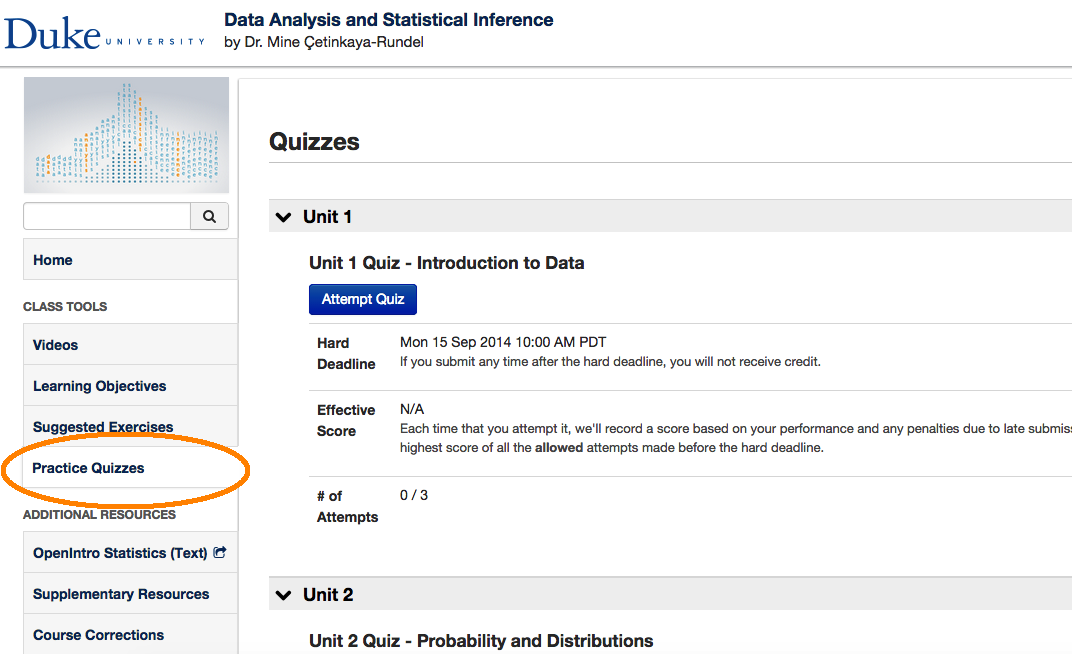
\includegraphics[width=0.6\textwidth]{figures/coursera_quiz}
\end{center}

\item PA3 will be posted on Monday after class and will be due that evening, so budget your time accordingly for that short turnaround!

\end{itemize}
% ALT ALT
% \begin{itemize}

% \item Exam 1 next Thursday (2/19)

% \item Sample exam + review questions posted on \webLink{\CourseSite}{course site} (on Feb 19 line)

% \item Additional practice quizzes on Coursera
% \begin{center}
% 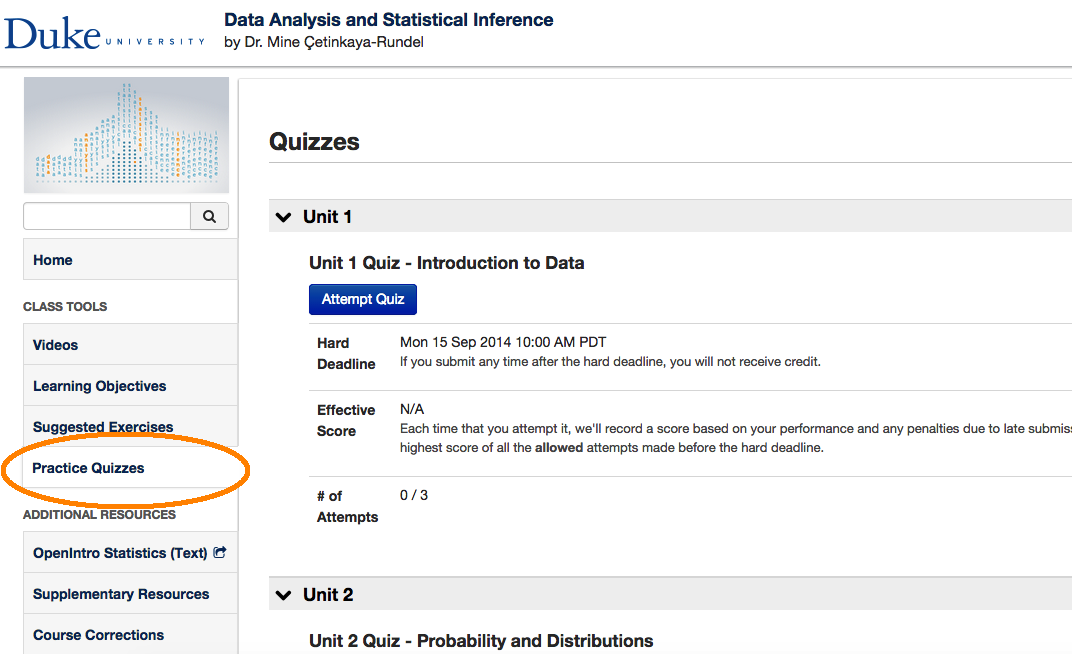
\includegraphics[width=0.6\textwidth]{figures/coursera_quiz}
% \end{center}

% \item PA3 will be posted on Tuesday after class and will be due Wednesday at
%   6pm.

% \end{itemize}

%---Note---%
\note{

}

\end{frame}

%%%%%%%%%%%%%%%%%%%%%%%%%%%%%%%%%%%%

\section{Main ideas}

\subsection{Statistical inference methods based on the CLT depend on the same conditions as the CLT}
\label{mi1}

%%%%%%%%%%%%%%%%%%%%%%%%%%%%%%%%%%%%

\begin{frame}
\frametitle{1. Statistical inference methods based on the CLT depend on the same conditions as the CLT}


\begin{enumerate}


\item \hlGr{Independence:} Sampled observations must be independent. \\

\item \hlGr{Sample size/skew:} Population must be normal or sample size must be
  large.

\end{enumerate}

\end{frame}

%%%%%%%%%%%%%%%%%%%%%%%%%%%%%%%%%%%%

\subsection{Statistical inference methods based on the CLT depend on the same conditions as the CLT}
\label{mi1}

% ALT ALT Commented out subsection above and frame below.

%%%%%%%%%%%%%%%%%%%%%%%%%%%%%%%%%%%%

\begin{frame}
\frametitle{1. Statistical inference methods based on the CLT depend on the same conditions as the CLT}

Always check these in context of the data and the research question!

\begin{enumerate}

\item \hlGr{Independence:} Sampled observations must be independent. \\

$\:$ \\
This is difficult to verify, but is more likely if
\begin{itemize}
\item random sampling/assignment is used, and,
\item if sampling without replacement, $n$ $<$ 10\% of the population.
\end{itemize}

\item \hlGr{Sample size/skew:} Either the population distribution is normal \\
or\\
$n > 30$ and the population distribution is not extremely skewed (the more skewed the distribution, the higher $n$ necessary for the CLT to apply).\\
$\:$ \\
This is also difficult to verify for the population, but we can check it using the sample data, and assume that the sample mirrors the population.

\end{enumerate}

%---Note---%
\note{

- Expect you to understand concepts.  Do you understand concept of independence.

}

\end{frame}

%%%%%%%%%%%%%%%%%%%%%%%%%%%%%%%%%%%%

\subsection{Use confidence intervals to estimate population parameters}
\label{mi2}

%%%%%%%%%%%%%%%%%%%%%%%%%%%%%%%%%%%%

\begin{frame}
\frametitle{2. Use confidence intervals to estimate population parameters}

\vfill

\[ CI: point~estimate \pm margin~of~error \]
$\:$ \\

\pause

If the parameter of interest is the population mean, and the point estimate is the sample mean,
\[ \bar{x} \pm Z^\star \frac{s}{\sqrt{n}} \]

\vfill

%---Note---%
\note{

1:36

- This is standard error of sample mean.

}

\end{frame}

%%%%%%%%%%%%%%%%%%%%%%%%%%%%%%%%%%%%

\begin{frame}

\vfill

\app{3.1 Confidence interval for a single mean}{See course website for details.}

\vfill

%---Note---%
\note{

- Give 10 minutes.

- Take students about 15 to finish.

- Popluation distribution, sample distribution, sampling distribution

- Took about 15 minutes to discuss.

}

\end{frame}

%%%%%%%%%%%%%%%%%%%%%%%%%%%%%%%%%%%%

\subsection{Critical value depends on the confidence level}
\label{mi3}

%%%%%%%%%%%%%%%%%%%%%%%%%%%%%%%%%%%%

\begin{frame}
\frametitle{3. Critical value depends on the confidence level}

\clicker{What is the critical value ($Z^\star$) for a confidence interval at the 91\% confidence level?}

\twocol{0.4}{0.6}{
\begin{enumerate}[(a)]
\item $Z^\star = 1.34$
\item $Z^\star = 1.65$
\item \solnMult{$Z^\star = 1.70$}
\item $Z^\star = 1.96$
\item $Z^\star = 2.33$
\end{enumerate}
}
{
\pause
\soln{
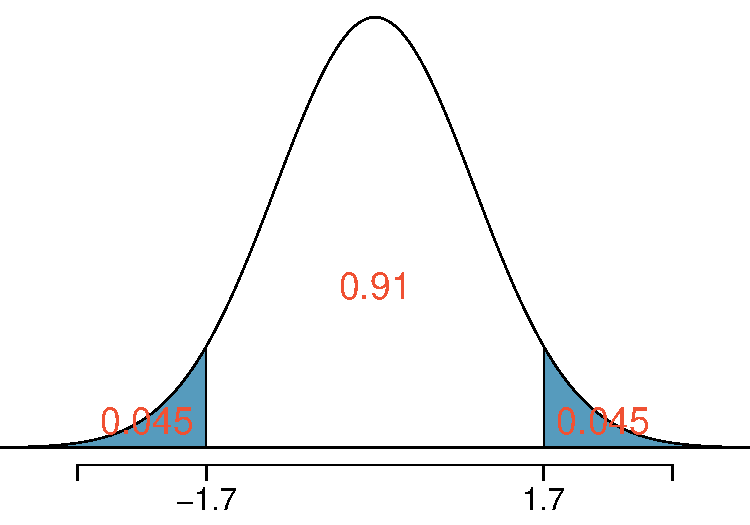
\includegraphics[width=\textwidth]{figures/conf_level/conf_level}
}
}

%---Note---%
\note{

- Look up using back of the book.

- People will mess this up.

- Given them time to discuss.

- People mess up again.

- May need to go over a bit and give them one more try.

}

\end{frame}

%%%%%%%%%%%%%%%%%%%%%%%%%%%%%%%%%%%%

\begin{frame}
\frametitle{Common misconceptions about confidence intervals}

\begin{enumerate}

\item \textcolor{gray}{The confidence level of a confidence interval is the
    probability that \textbf{the specific confidence interval you construct
      after gathering a sample} contains the true population parameter.} \\
\textit{This is incorrect, CIs are part of the frequentist paradigm and as such the population parameter is fixed but unknown. Consequently, the probability any given CI contains the true value must be 0 or 1 (it does or does not).} \\
$\:$ \\

\pause

\item  \textcolor{gray}{A narrower confidence interval is always better.}\\
\textit{This is incorrect since the width is a function of both the confidence level and the standard error.} \\
$\:$ \\

\pause

\item   \textcolor{gray}{A wider interval means less confidence.} \\
\textit{This is incorrect since it is possible to make very precise statements with very little confidence.} \\

\end{enumerate}

%---Note---%
\note{

- Distinction: The confidence interval you construct once does or does not
contain the true popultion mean.  This is an a priori thing.

}

\end{frame}

% ALT ALT

% Commented out above.  Created below.

%%%%%%%%%%%%%%%%%%%%%%%%%%%%%%%%%%%%

% \begin{frame}
% \frametitle{Common misconceptions about confidence intervals}

% \begin{enumerate}

% \item \textcolor{gray}{The confidence level of a confidence interval is the
%     probability that the true pop.\ parameter is in the confidence
%     interval you construct \textbf{for a single sample}.} \\
%   \textit{The confidence level is equal to the proportion of random samples that result
%     in confidence intervals that contain the true pop.\ parameter.} \\
%   $\:$ \\

% \pause

% \item  \textcolor{gray}{A narrower confidence interval is always better.}\\

% \item   \textcolor{gray}{A wider interval means less confidence.} \\

% \hfill \\

% \textit{The width is a function of both the \textbf{confidence level} and \textbf{the standard error}.} \\

% \end{enumerate}

% %---Note---%
% \note{

% - Distinction: The confidence interval you construct once does or does not
% contain the true popultion mean.  This is an a priori thing.

% }

% \end{frame}

%%%%%%%%%%%%%%%%%%%%%%%%%%%%%%%%%%%%

\subsection{Use hypothesis tests to make decisions about population parameters}
\label{mi4}

%%%%%%%%%%%%%%%%%%%%%%%%%%%%%%%%%%%%

\begin{frame}
\frametitle{4. Use hypothesis tests to make decisions about population parameters}

Hypothesis testing framework:

\begin{enumerate}

\item Set the hypotheses.

\item Check assumptions and conditions.

\item Calculate a \hl{test statistic} and a p-value.

\item Make a decision, and interpret it in context of the research question.

\end{enumerate}

\end{frame}

%%%%%%%%%%%%%%%%%%%%%%%%%%%%%%%%%%%

\begin{frame}
\frametitle{Hypothesis testing for a population mean}

\begin{enumerate}

\item Set the hypotheses
\begin{itemize}
\item $H_0: \mu = null~value$
\item $H_A: \mu <$ or $>$ or $\ne null~value$
\end{itemize}

\pause

\item Check assumptions and conditions
\begin{itemize}
\item Independence: random sample/assignment, 10\% condition when sampling without replacement
\item Sample size / skew: $n \ge 30$ (or larger if sample is skewed), no extreme skew
\end{itemize}

\pause

\item Calculate a \hl{test statistic} and a p-value (draw a picture!)
\[ Z = \frac{\bar{x} - \mu}{SE},~where~SE = \frac{s}{\sqrt{n}} \]

\pause

\item Make a decision, and interpret it in context of the research question
\begin{itemize}
\item If p-value $< \alpha$, reject $H_0$, data provide evidence for $H_A$
\item If p-value $> \alpha$, do not reject $H_0$, data do not provide evidence for $H_A$
\end{itemize}

\end{enumerate}

\end{frame}

%%%%%%%%%%%%%%%%%%%%%%%%%%%%%%%%%%%%

\begin{frame}
\frametitle{4. Use hypothesis tests to make decisions about population parameters}

\vfill

\app{3.2 Hypothesis testing for a single mean}{See course website for details.}

\vfill

\end{frame}

%%%%%%%%%%%%%%%%%%%%%%%%%%%%%%%%%%%%

\begin{frame}

\clicker{Which of the following is the correct interpretation of the p-value
  from App Ex 3.2?}

\begin{enumerate}[(a)]
\item The probability that average GPA of Duke students has changed since 2001.
\item The probability that average GPA of Duke students has not changed since 2001.
\item The probability that average GPA of Duke students has not changed since 2001, if in fact a random sample of 63 Duke students this year have an average GPA of 3.58 or higher.
\item The probability that a random sample of 63 Duke students have an average GPA of 3.58 or higher, if in fact the average GPA has not changed since 2001.
\item \solnMult{The probability that a random sample of 63 Duke students have an average GPA of 3.58 or higher or 3.16 or lower, if in fact the average GPA has not changed since 2001.}
\end{enumerate}

\end{frame}

%%%%%%%%%%%%%%%%%%%%%%%%%%%%%%%%%%%%

\begin{frame}
\frametitle{Common misconceptions about hypothesis testing}

\begin{enumerate}

\item \textcolor{gray}{P-value is the probability that the null hypothesis is true} \\
\textit{This is incorrect, p-value is the probability of the observed or more extreme outcome if in fact the null hypothesis is correct. It is the conditional probability of the observed data (or something more extreme), conditioned on the null hypothesis being correct.} \\
$\:$ \\

\pause

\item  \textcolor{gray}{A high p-value confirms the null hypothesis.}\\
\textit{This is incorrect, a high p-value means the data do not provide convincing evidence for the alternative hypothesis and hence that the null hypothesis can't be rejected.} \\
$\:$ \\

\pause

\item   \textcolor{gray}{A low p-value confirms the alternative hypothesis.} \\
\textit{This is incorrect, a low p-value means the data provide convincing evidence for the alternative hypothesis, but not necessarily that it is confirmed.} \\

\end{enumerate}

\end{frame}

% ALT ALT

% \begin{frame}
% \frametitle{Common misconceptions about hypothesis testing}

% \begin{enumerate}

% \item \textcolor{gray}{P-value is the probability that the null hypothesis is true} \\
%   \textit{\small A p-value is the probability of getting a sample that results in a
%     test statistic as or more extreme than what you actually observed (and in
%     favor of the null hypothesis) if in fact the null hypothesis is correct. It is a conditional probability, conditioned on the null hypothesis being correct.} \\
%   $\:$ \\

% \pause

% \item  \textcolor{gray}{A high p-value confirms the null hypothesis.}\\
% \textit{A high p-value means the data do not provide convincing evidence for the alternative hypothesis and hence that the null hypothesis can't be rejected.} \\
% $\:$ \\

% \pause

% \item   \textcolor{gray}{A low p-value confirms the alternative hypothesis.} \\
% \textit{A low p-value means the data provide convincing evidence for the alternative hypothesis, but not necessarily that it is confirmed.} \\

% \end{enumerate}

% \end{frame}


%%%%%%%%%%%%%%%%%%%%%%%%%%%%%%%%%%%%

\section{Summary}

%%%%%%%%%%%%%%%%%%%%%%%%%%%%%%%%%%%%

\begin{frame}
\frametitle{Summary of main ideas}

\vfill

\begin{enumerate}

\item \nameref{mi1}
% ALT ALT

\item \nameref{mi2}

\item \nameref{mi3}

\item \nameref{mi4}

\end{enumerate}

\vfill

\end{frame}

%%%%%%%%%%%%%%%%%%%%%%%%%%%%%%%%%%%

\end{document}